\chapter{Background}\label{chapter:background}

This chapter introduces the concepts that make the building blocks for our
iptables model, making use of the extensive work conducted by Stoenescu et
al.~\cite{stoenescu2013symnet, stoenescu2016symnet}

We first give a short overview of the broad field of network verification, with
an emphasis on the approach that we use: static verification powered by
symbolic execution.  We then show how it is implemented in SymNet, and how
SymNet can be used to verify the models we build.  Finally, we cover iptables
in detail; we discuss its internal organization, as well as its most common
features.


\section{Network verification}\label{sec:network-verification}
Formal verification is the act of proving or disproving the correctness of
intended algorithms underlying a system with respect to a certain formal
specification or property using formal methods of
mathematics~\cite{sanghavi2010formal}. Network verification is merely formal
verification tailored for network-related questions.

\paragraph{Correctness.}\label{par:correctness}
But in order to apply it, we first need to provide a rigorous definition for
network correctness.  It turns out that this is by itself a very involved task.
Being abstract is what one might try in order to get around this formalism:

\begin{definition}[Network correctness]
\label{def:full-correctness}
A network behaves correctly as long as it complies to operator's policy.
\end{definition}

At first, this definition does not seem to accomplish much, as what it
essentially does is to delegate the requirement by introducing the need to
formally define a \emph{policy}, or, more precisely, its composing rules.
Therefore, the follow-up question that arises is:

\begin{quote}
What is a (policy) rule and how is it specified?
\end{quote}

In fact, there is ongoing work that focuses on bringing policy specification
closer to the natural language and using the resulting format to automate
policy proving.  This novel technique, called \textbf{policy-driven network
verification}, could significantly reduce verification run-times, similar to
the way \emph{informed search} algorithms compare to the uninformed ones on
large search spaces.  Another analogy stems from the field of automatic theorem
proving: policy-based verification resembles the \emph{forward chaining}
inference method, by propagating packets through the modelled network (a
procedure further detailed in \labelindexref{Section}{sub-sec:symb-exec}) until
either the policy is proved or a contradiction is reached.

A complementary approach, rather than an alternative, which proves more
practical by circumventing the need for a correctness definition that covers
all desired properties is to specialize the verification to specific goals.
So, instead of a \emph{proper} correctness definition, we could define multiple
\emph{partial} ones, such as:

\begin{definition}[Partial network correctness - Reachability]
If the network behaves correctly, then nodes A and B should be reachable from
one another.
\end{definition}

\begin{definition}[Partial network correctness - Encrypted traffic]
If the network behaves correctly, then TCP (Transmission Control
Protocol)\abbrev{TCP}{Transmission Control Protocol} traffic between Alice
and Bob should be encrypted.
\end{definition}

Notice the \hlmath{$correctness \implies property$} form, instead of
\hlmath{$correctness \iff policy$}, in
\labelindexref{Definition}{def:full-correctness}.  Still, using simple logic
rules, if we admit that the policy is a conjunction of rules (i.e. properties),
\hlmath{$P = r_1 \wedge r_2 \wedge ... \wedge r_n$}, and we prove
\hlmath{$r_i$, $\mbox{for } i = 1,...,n$}, then
\hlmath{$correctness \implies P$}.  Since the reverse implication is true by
definition, this yields the same equivalence.  Therefore, by decomposing the
policy into its defining rules not only do we get an easier to implement
verification system, but we also reach the same theoretical result, provided
that all rules are known.  In addition to that, policy specification is an
iterative process in practice, making this approach even more desirable.

\paragraph{Modelling and verification procedure.}
The other two essential ingredients needed to apply formal verification to
networking problems are a model of the network and a specific procedure for
proving or disproving its correctness.  The model is an abstract (i.e.
mathematical) representation of the network that can be easily handled by the
proof procedure.

The most well-established proof procedure is \textbf{model
checking}~\cite{clarke1999model, mcmillan2003model} which does an exhaustive
exploration of the states a system can be in to verify that a given property
holds. Another technique which has been thoroughly explored is
\textbf{reduction to SAT} (AntEater~\cite{mai2011debugging}).  However, for
large models that result even from moderately sized networks the aforementioned
approaches render the verification problem intractable.  Other
modelling/verification techniques which have been considered over time are the
following:
\begin{itemize}
  \item Modelling the network as a \textbf{distributed system}, where each
    network element (i.e. computing node) has its own corresponding \emph{C
    code}, and then running symbolic execution (discussed in
    \labelindexref{Section}{sub-sec:symb-exec}) on it.  This approach has two
    major downsides:
      \begin{enumerate}[(i)]
        \item Currently, symbolic execution rapidly reaches its worst-case
          exponential complexity when run on large C programs, and
        \item Having to consider all possible interleavings of different
          threads, as in any other parallel model, makes it unsuitable even
          for small C programs.
      \end{enumerate}
  \item Creating a simplified model of both the \textbf{control plane} and the
    \textbf{data plane} of each network element and simulate their interactions
    (\labelindexref{Figure}{fig:control-data-verif}).  However, modelling the
    control plane is hard to achieve in practice, because:
    \begin{enumerate}[(i)]
      \item Many processes that are part of it are asynchronous, which means
        that they inherit all the downsides of modelling distributed systems;
        examples include dynamic routing protocols updates and SDN
        (Software-defined networking)\abbrev{SDN}{Software-Defined Networking}
        controller updates.
      \item Building on the previous one, control planes are usually very
        complex, especially since more and more middleboxes become fundamental
        in today's networks.  One way to simplify the process of modelling it
        is to specialize the model for one particular process
       ~\cite{weitz2016bagpipe, fogel2015general}, but this loses generality.
    \end{enumerate}
  \item Model only the data plane of the network in such a way that processing
    logic which does not affect packet flows is ignored
    (\labelindexref{Figure}{fig:control-data-verif}).  When combined with
    \textbf{symbolic execution}, the result is a scalable
    \textbf{static data plane verification} approach that features one of the
    best trade-offs between model accuracy and verification complexity.
    Therefore, it is further discussed in the next two sections.
\end{itemize}

\begin{figure}[h]
  \centering
  \captionsetup{justification=centering}
  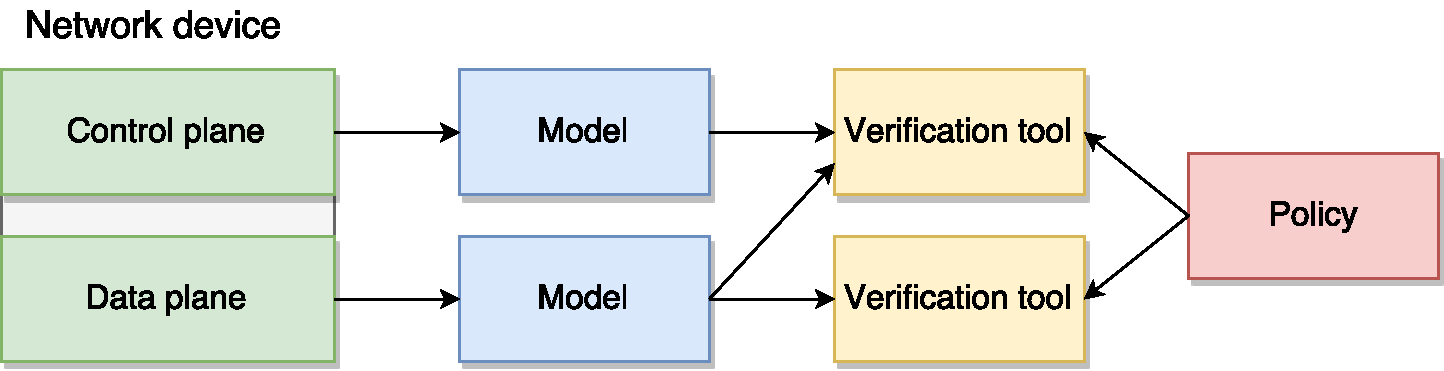
\includegraphics[scale=0.5]{assets/img/control-data}
  \caption{Data plane verification vs. control plane \emph{and} data plane
  verification.}
  \label{fig:control-data-verif}
\end{figure}

It is also worth briefly introducing one of the primary alternatives to
model-based static network verification, \textbf{Dynamic Network Testing} (also
known as \emph{packet injection}). As a testing technique, rather than a formal
verification one, it runs on the actual network infrastructure in a specially
configured, isolated environment.  Some network hosts, called \emph{test
agents}, generate traffic according to some test cases and evaluate the results
of each network element that is subject to testing.  However, its downsides
greatly overweight its advantages:

\begin{itemize}
  \item The search space is implicitly defined by the test cases, which means
    that a good coverage corresponds to a(n) (exponentially) large number of
    tests.
  \item Adding to the previous point, there is an inherent bias introduced by
    having the test cases cover commonly observed behaviours, without exploring
    unexpected ones, which might lead to failures.
  \item Overall, it is more expensive to perform and requires more resources
    than static analysis.
\end{itemize}


\subsection{Static data plane verification}\label{sub-sec:static-dp-verif}

Starting from the observation that including control planes in our models with
the end goal of verifying multiple properties of large (i.e.  enterprise-size)
networks does not scale, we are left with the smaller part of each network
device: its data plane (\labelindexref{Figure}{fig:data-plane-snapshot}).

\begin{figure}[h]
  \centering
  \captionsetup{justification=centering}
  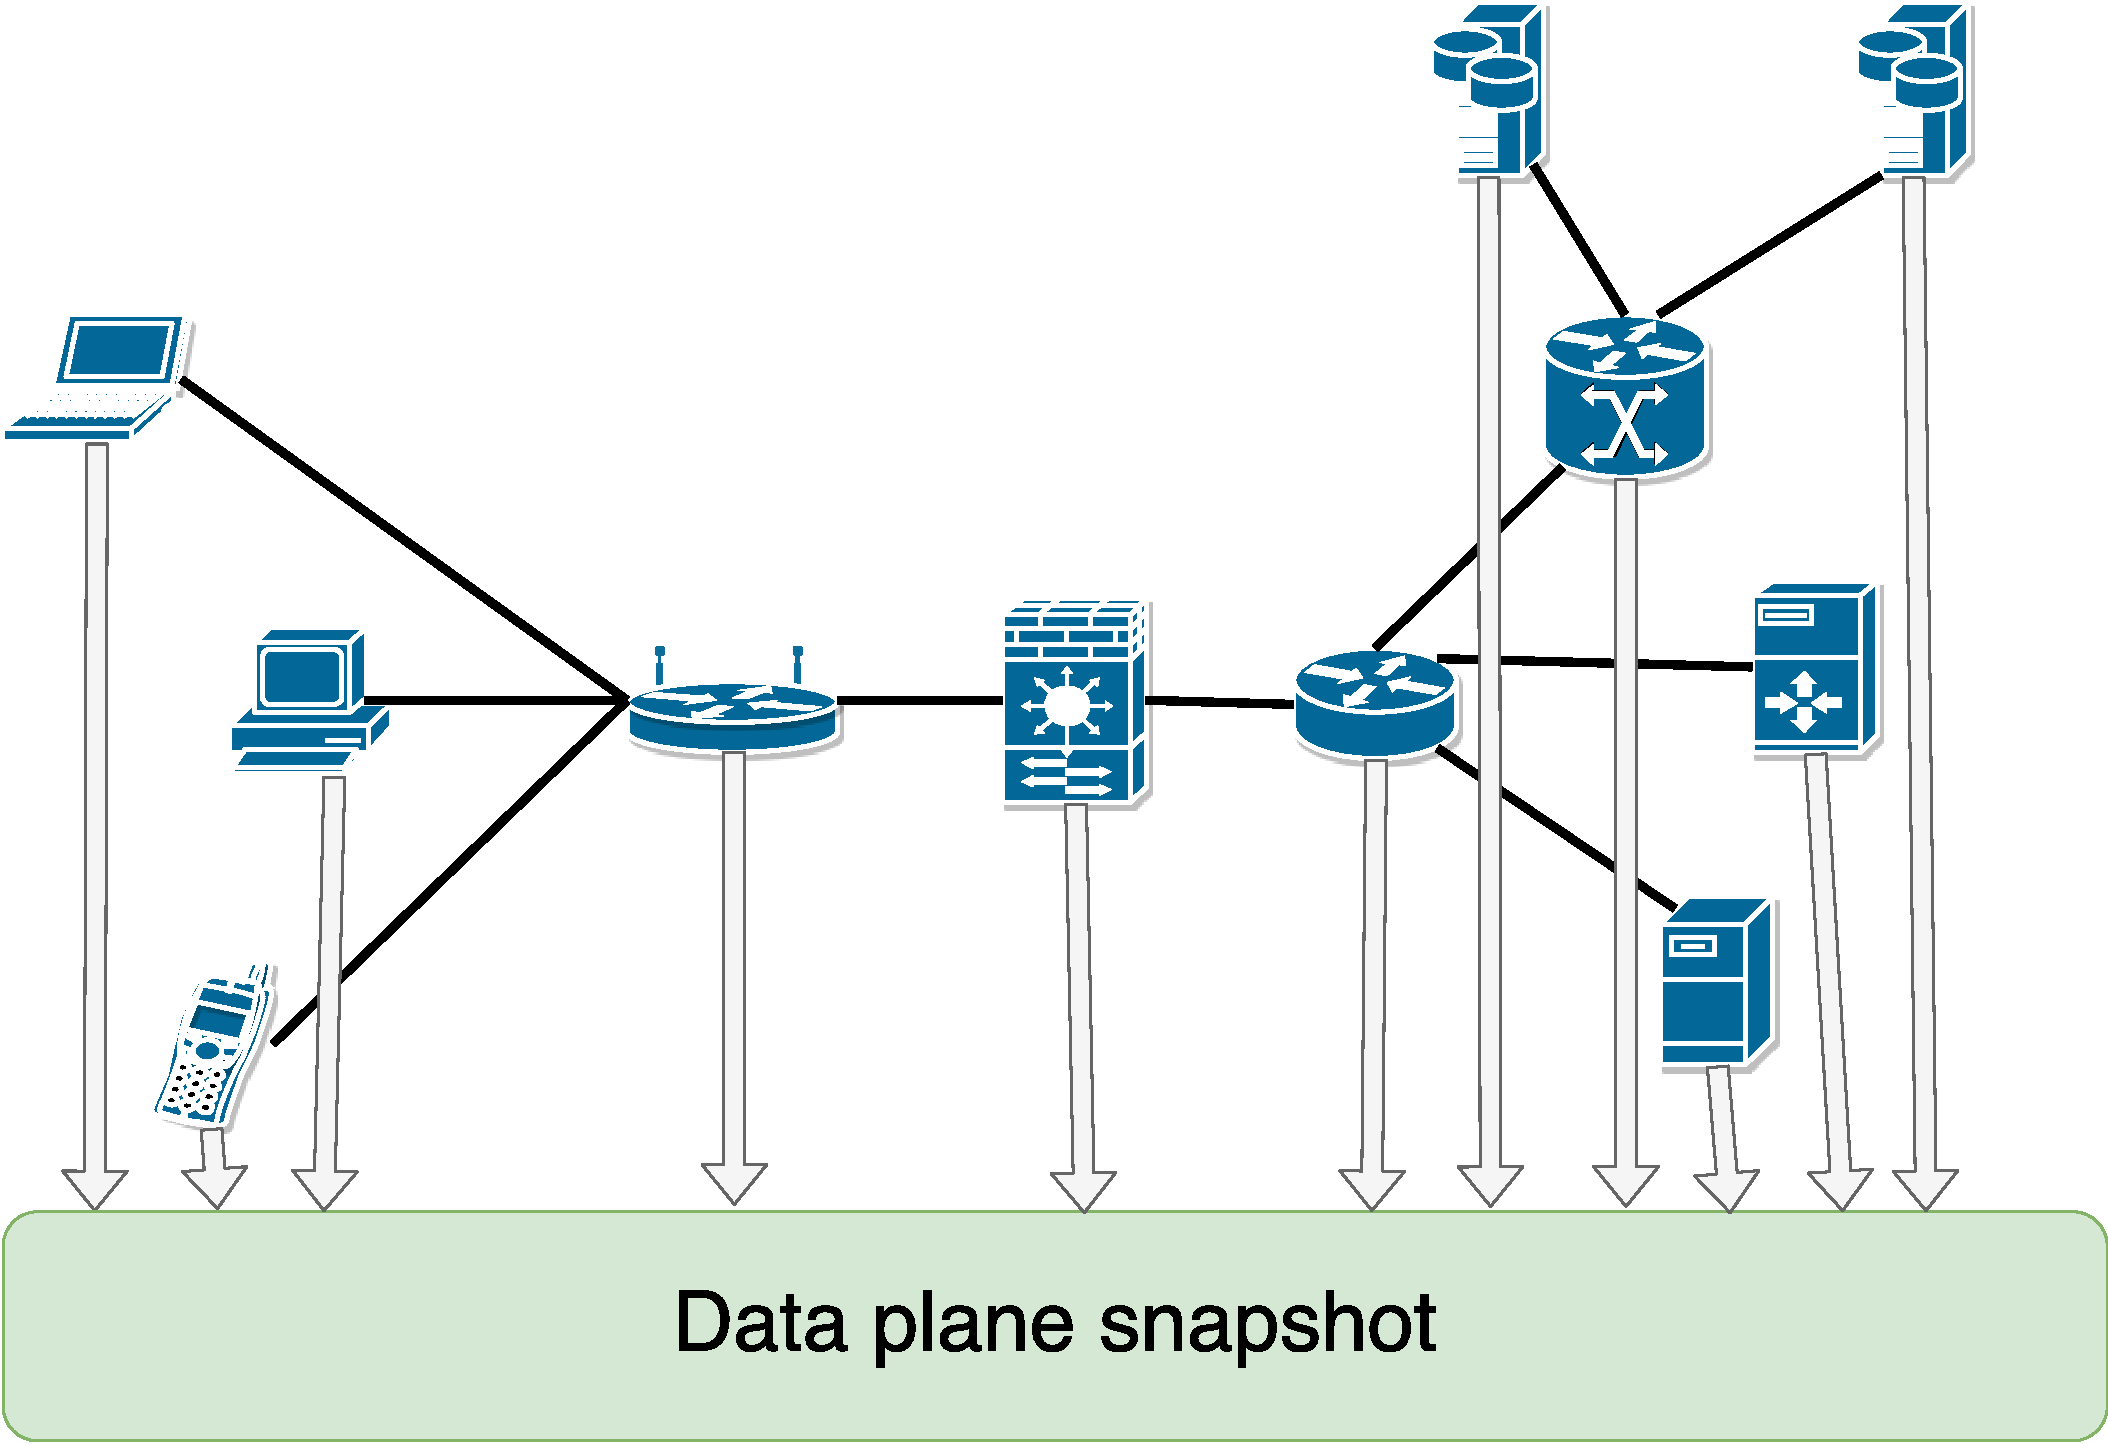
\includegraphics[scale=0.3]{assets/img/data-plane-snapshot}
  \caption{Data plane/control plane decoupling.}
  \label{fig:data-plane-snapshot}
\end{figure}

Data planes (often \textbf{forwarding planes}) include only the \emph{rules}
needed by devices to expose the functionality they are designed for.  For
example, the data plane of a router is represented by its routing table, and,
possibly, packet filtering ACLs (Access Control Lists)\abbrev{ACL}{Access
Control List}.  A switch takes its decisions based on the MAC\abbrev{MAC}{Media
Access Control} table. Both of these tables are specific instances of the more
general Forwarding Information Base (FIB)\abbrev{FIB}{Forwarding Information
Base}, a name that refers to the specialized hardware components responsible
for forwarding in various network devices.

Limiting the models to network data planes can be interpreted in two
contradictory ways:
\begin{enumerate}[(i)]
  \item As a downside, for ignoring the other half that makes up a network
    device: its rule-making processes, the control plane.
  \item As an approach that enables scalable verification, based on the insight
    that, even if short-lived, the data plane of a network is what dictates its
    operation at an instant.
\end{enumerate}

The second point constitutes the motivation behind the framework described in
\labelindexref{Section}{sec:symnet-sefl}.  Another way of looking at it is that
we simply ignore any process that leads to the current network
\emph{configuration} and establish whether it is a correct one or not.  If it
is, then an incremental analysis can be applied from that point forward: this
implies analyzing only the updates that reach the data plane, a technique which
has already been studied in the parent field of software
verification~\cite{marinescu2013katch}.  If our initial verification reports
failure, human intervention is required in order to detect the control plane
problem that caused the unexpected rule in the data plane.


\subsection{Symbolic execution}\label{sub-sec:symb-exec}

Symbolic execution is a means of statically analyzing a program in order to
find the inputs that cause certain parts of it to be executed.  It results in a
tree with each node representing a possible state in its execution, and edges
corresponding to state transitions caused by executing the next instruction on
that specific path.  Therefore, execution paths in the analyzed program
correspond to state chains starting from the root of the symbolic execution
tree.  A state, in this context, is a collection of variables together with
their constraints expressed in terms of symbolic inputs of the program and/or
other variables.

To clarify things, let us step through a concrete example and highlight the
construction of the symbolic execution tree
(\labelindexref{Figure}{fig:simple-tree}) for a simple C function
(\labelindexref{Listing}{lst:simple-c}):
\begin{itemize}
  \newcommand{\pa}{\hltexttt{a}}
  \newcommand{\pb}{\hltexttt{b}}
  \newcommand{\pc}{\hltexttt{c}}
  \newcommand{\vmax}{\hltexttt{max}}

  \item We assume that the \hltexttt{max3} function can be called with any
    integer arguments.  Thus, its formal parameters \pa{}, \pb{} and \pc{} are
    the input of this symbolic execution; they are assigned
    pure\footnote{In this context, \emph{pure} is synonymous with
    \emph{unconstrained}.} \emph{symbolic values} denoted by Greek letters
    $\alpha$, $\beta$ and $\gamma$, and together constitute the initial state
    (i.e. the root node in the symbolic execution tree).  Implementation-wise,
    symbolic values can be represented as full ranges given by their underlying
    types on the machine model that is targeted (e.g.  $[-2.147.483.648;
    +2.147.483.647]$ for a 4-bytes signed integer).

  \item At \textbf{line 3}, a new variable, \vmax{}, is defined.  This is where
    language-specific behaviour comes into play, as we use the fact that the
    value of an uninitialized variable allocated on the stack is
    unspecified\footnote{From the ISO/IEC 9899:2011 standard, informally
    \textbf{C11}, paragraph \textbf{3.19.3 unspecified value} says: \emph{valid
    value of the relevant type where this International Standard imposes no
    requirements on which value is chosen in any instance}.} and we accordingly
    assign it a symbolic value.

    Note that in \labelindexref{Figure}{fig:simple-tree} variable \vmax{} is
    added to the root node due to lack of space; formally, there should be a
    transition between the initial state (described above) and the state where
    it gets introduced.

\begin{minipage}{.45\textwidth}
\begin{listing}[H]
  \sourcecode{c}{assets/code/simple-c.c}
  \caption{Simple C function used to visualize symbolic execution.}
  \label{lst:simple-c}
\end{listing}
\end{minipage}\hfill
\begin{minipage}{.45\textwidth}
  \centering
  \captionsetup{justification=centering}
  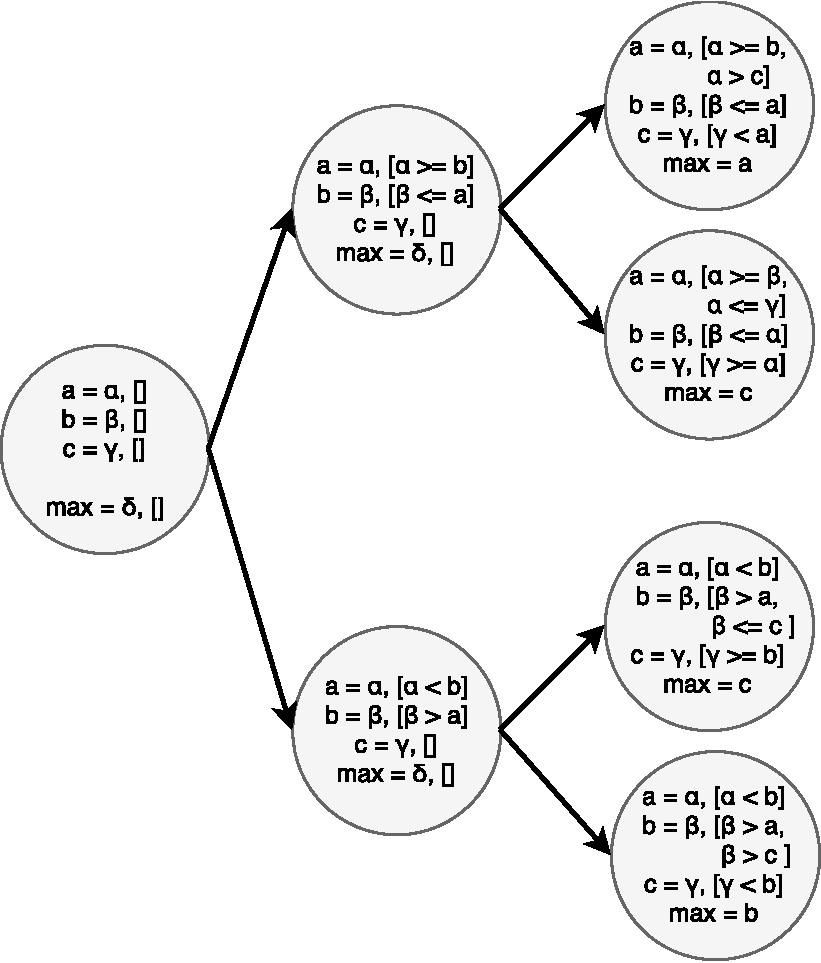
\includegraphics[scale=0.49]{assets/img/symb-tree}
  \captionof{figure}{Symbolic execution tree for the C function in
    \labelindexref{Listing}{lst:simple-c}.}
  \label{fig:simple-tree}
\end{minipage}

  \item At \textbf{line 5}, the first \hltexttt{if/then/else} statement is
    reached causing the current state to \emph{fork}; this creates two child
    nodes that correspond to the two possible scenarios: following the
    \hltexttt{then} part, which means that the condition is true, and following
    the \hltexttt{else} part, corresponding to its negation being true.  Notice
    that constraints are added to both variables \pa{} and \pb{} in each of the
    new states, using antisymmetry.

  \item Similar to the previous step, at \textbf{lines 7 and 12} the inner
    \hltexttt{if/then/else} statements are symbolically executed yielding four
    more states, as well as two more constraints in each one of them.

    The interesting bit here is that variable \vmax{} loses its previously
    assigned symbolic value, $\delta$, together with its \textbf{constraints}
    (which happens to be an empty list in this example) once it is assigned one
    of \pa{}, \pb{} or \pc{}.  It also inherits all their constraints, which is
    not explicitly highlighted in \labelindexref{Figure}{fig:simple-tree}.
\end{itemize}

We can derive a couple of properties for symbolic execution even from such a
small example:
\begin{enumerate}[a)]
  \item On the \textbf{upside}, it enables \emph{invariant checking} by
    ensuring that certain properties hold in all explored states, and, thus,
    are true irrespective of input.  Furthermore, it can help increase code
    coverage\footnote{Code coverage is a measure used to described the degree
    to which the source code of a program is executed when a particular test
    suite runs.} by generating unit tests that explore previously untouched
    parts of the program.

  \item On the \textbf{downside}, it commonly leads to \textbf{path explosion},
    which is arguably its single most limiting factor. Path explosion refers to
    the exponential increase in the number of states (and, implicitly, paths)
    in the symbolic execution tree as the number of traversed \emph{conditional
    branches} in the program accumulate. Even though heuristic methods to
    reduce time and/or space have been devised (e.g. parallelizing independent
    paths~\cite{staats2010parallel}, merging similar
    paths~\cite{kuznetsov2012efficient}, etc), it still remains a concern.

    That being said, it is worth stressing that it is not the \emph{length} of
    the analyzed program that causes path explosion, but certain types of
    instructions: conditional branches.  This is an important remark which
    becomes meaningful when used to guide the design of a DSL (Domain Specific
    Language)\abbrev{DSL}{Domain Specific Language} that aims to be
    \emph{symbolic execution friendly}, introduced in the following section.
\end{enumerate}


\section{SymNet and SEFL}\label{sec:symnet-sefl}

SymNet and SEFL establish together the framework we use to model and verify
large, complex, stateful networks. SymNet is a network analysis tool that
accepts as input a (SEFL) model of the network which is subject to
verification, and uses symbolic execution to find all possible packet flows
that might traverse it.  SEFL is a network processing DSL that describes
network functions as flow transformations.  Even though they serve conceptually
different purposes, they have been designed and optimized to be used together.
Therefore, it is common to refer to the system as a whole through
\emph{``SymNet''}.

The \textbf{key novelty} of this network verification system is making the
verification procedure (that is, symbolic execution) a core part of the design
behind the network description language that it uses (and even name it).  Thus,
careful crafting of SEFL models can keep \emph{path explosion}
under control and achieve performances unreached before: it has been used to
verify backbone routers with hundreds of thousands of prefixes in
seconds~\cite{stoenescu2016symnet}, and has been shown to scale linearly with
the size of the analyzed network~\cite{stoenescu2013symnet}.

\begin{figure}[h]
  \centering
  \captionsetup{justification=centering}
  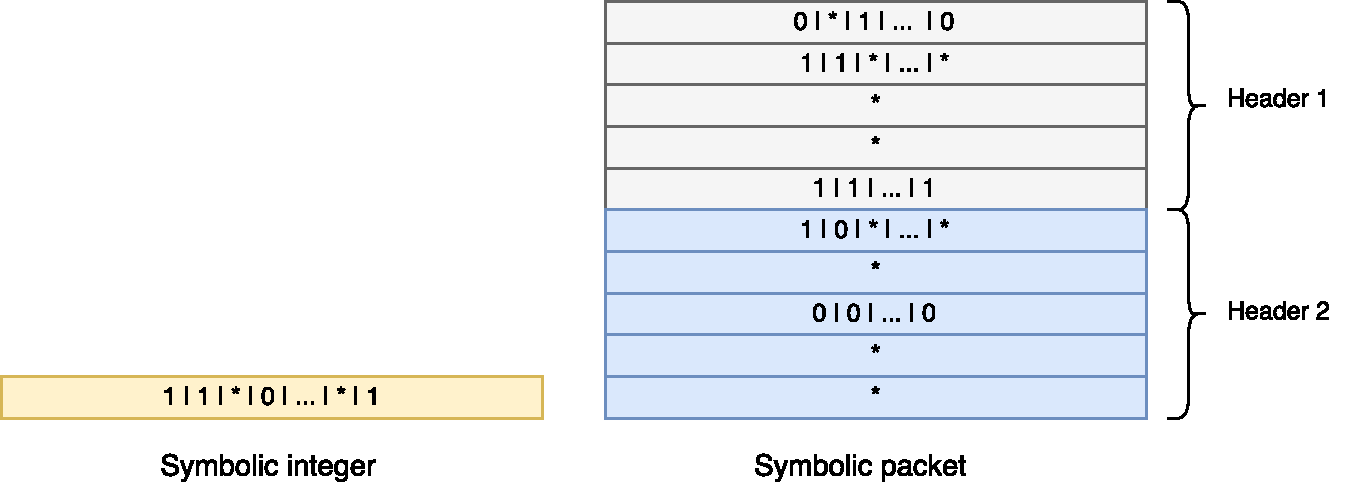
\includegraphics[scale=0.6]{assets/img/symbolic-packet}
  \caption[Visualization of a symbolic integer value and a symbolic
  packet]{Visualization of a symbolic integer value and a symbolic packet.
  Stars (\textbf{*}) are used to denote symbolic fields and bits.}
  \label{fig:symbolic-packet}
\end{figure}

\paragraph{Modelling packets.}
Packets are to SymNet how variables are to regular symbolic execution tools
(e.g. KLEE~\cite{cadar2008klee}). The main difference is that instead of a
4-bytes signed integer, for instance, a packet is a collection of
\emph{headers}, and each header is a collection of \emph{header fields},
similar to real implementations (\labelindexref{Figure}{fig:symbolic-packet}).
The common symbolic execution terminology is also inherited: \emph{symbolic}
packet, \emph{symbolic} header field, \emph{constrained} header field,
\emph{concrete} packet, etc.

To continue the analogy, SEFL instructions are similar to usual instructions in
a C program.  However, in SEFL, instructions implicitly operate on the header
fields of a single packet; that is, the memory space is a packet (or, more
precisely, a \emph{packet flow}, as we will shortly see).  Therefore, another
defining design aspect behind SymNet is that a packet is tied to a symbolic
execution path.

Another novel capability of SymNet is modelling \textbf{stateful} network
devices.  This is achieved by adding per-flow state as additional dimensions in
the packet header.  It includes all state information which would normally
reside on the stateful devices that are traversed.

\begin{figure}[h]
  \centering
  \captionsetup{justification=centering}
  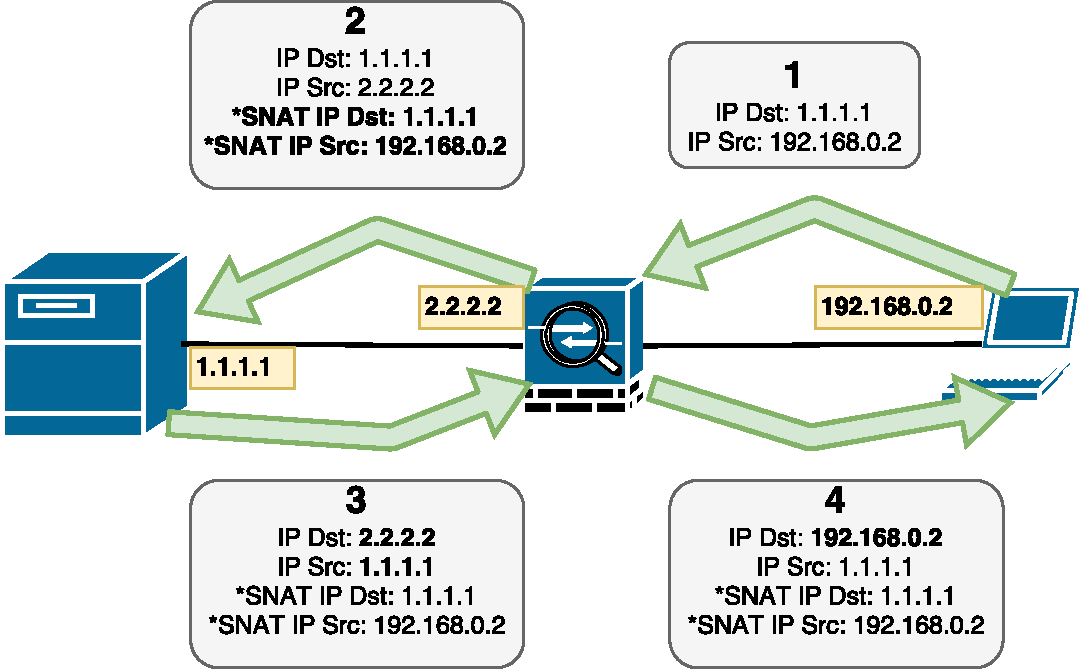
\includegraphics[scale=0.6]{assets/img/snat-example}
  \caption{Packet flow during connection initiation and reply while behind a
  NAT appliance.}
  \label{fig:snat-example}
\end{figure}

An example of how this works is presented in
\labelindexref{Figure}{fig:snat-example}.  The user on the right initiates a
connection with the server on the left \textbf{(1)}.  He is behind a NAT
appliance which is configured to SNAT (Source NAT) outgoing connections.  Since
the 5-tuples identifying address translations are stored by the NAT box, we
model its logic in SEFL by adding this information as part of the flow. Due to
lack of space, in this example we only include the source and the destination
IP addresses; the star in front of these new fields helps differentiate regular
header fields and state-related ones \textbf{(2)}.  The reply packet is part of
the same flow, so we make sure it keeps these fields unchanged \textbf{(3)}.
When the reply arrives at the NAT box, it uses the state fields to apply the
reverse translation and forward the packet to its original source \textbf{(4)}.

\bigskip

It is worth reiterating that SymNet fits into the static data plane
verification category since the models built using SEFL are solely based on the
data plane of each network element.  As already argued in
\labelindexref{Section}{sub-sec:static-dp-verif}, this technique proves to be a
good trade-off between model accuracy and verification complexity.  In many
formal verification systems the equivalence between the model and the target
system is enforced by construction.  However, in order to reach a tractable
problem, besides ignoring the control plane in the modelling process, SymNet
makes a few additional assumptions:
\begin{itemize}
  \item \textbf{Independence between different flows.} A consequence of
    storing the state of middleboxes as part of the flow and having SEFL focus
    on one flow only means that per-device global state is ignored.  This
    includes internal buffer sizes, seeds used for randomization, and various
    other statistics. There is also no notion of flow ordering, which might
    make a difference in practice.
  \item \textbf{The network is operationally correct.} Scenarios such as memory
    corruption and devices failing spuriously are not considered.
\end{itemize}


\subsection{Building network models with SEFL}\label{sub-sec:building-models}

A \textbf{network model} described using SEFL and processed by SymNet is a
directed graph, \hlmath{$G = (V, E)$}, with nodes \hlmath{$u\in V$}, often
called \textbf{ports}, that have SEFL instructions associated, and edges
\hlmath{$(u, v)\in E$} commonly referred to as \textbf{links}.  Additionally,
the following property holds: \hlmath{$\forall u\in V$, $deg^{+}(u) <= 1$}. In
other words, each node should have no more than one outgoing edge (i.e.
one-to-many relationships are not allowed). Otherwise, a form of
\textbf{implicit} non-determinism would result (i.e.  \emph{unconditional
fork}) which does not make sense in this context.  \textbf{Explicit} forks are
supported, as highlighted in \labelindexref{Table}{tab:sefl-instr} which is an
overview of the most common SEFL instructions.

\begin{table}
  \small
  \centering
  \begin{tabular}{ | l | p{10cm} |}
    \hline
    % Header.
    \textbf{Instruction} & \textbf{Description} \\ \hline

    % Constrain.
    Constrain(var, condition) & Adds \emph{condition} to the list of
    constraints for variable \emph{var}.  If it is unsatisfiable, the current
    execution path fails. Note that \emph{condition} is a predicate (i.e.
    boolean-valued function), or a conjunction/disjunction of predicates,
    generally expressed as a partially applied two-parameters boolean function
    in Polish notation.

    Example: Constrain("a", $== 10$), Constrain("b", $\land(> 10, < 12)$)
    \\ \hline

    % If.
    If (condition, then, else) & Forks the execution path, yielding two new
    packet flows: one continues on the \emph{then} branch iff.\
    \emph{condition} is satisfiable, and the other continues on the \emph{else}
    branch iff. its negation is satisfiable.  Note that conditions are
    expressed in terms of \emph{Constrain}.
    \\ \hline

    % Fail.
    Fail(message) & Explicitly stop symbolic execution for the current flow.
    Note that this is one of the instructions that are part of the language
    just to ease the interaction with the symbolic execution engine.
    \\ \hline

    % Forward.
    Forward(port) & Forwards this packet to \emph{port}.  Execution will
    continue starting with the instructions associated with it.
    \\ \hline

    % Fork.
    Fork(i1, i2, ...) & Explicitly forks the current execution path into a number of new
    flows and for each new flow $j$, continues execution with instruction
    $i_{j}$.
    \\ \hline

    % InstructionBlock.
    InstructionBlock(i1, i2, ...) & Acts as the \emph{composite} type in a
    composite design pattern; simply aggregates the given instructions and
    executes them in the specified order.
    \\ \hline

    % NoOp
    NoOp & This instruction is simply skipped by the symbolic execution engine.
    \\ \hline
  \end{tabular}
  \caption{Common SEFL instructions.}
  \label{tab:sefl-instr}
\end{table}

Note that many-to-one relationships are still possible. Therefore, while it is
natural to think of a link as a physical wire connecting two ports, they are
not limited to that, as it is shown in the example below.

So far we have seen \textbf{what} SEFL is capable of doing: model network
functions as packet flow transformations.  To illustrate
\textbf{how} this is accomplished by putting together all the pieces discussed
above, let us introduce the model of a simple router that only forwards packets
based on its routing table (\labelindexref{Figure}{fig:router-model}).

\begin{figure}[h]
  \centering
  \captionsetup{justification=centering}
  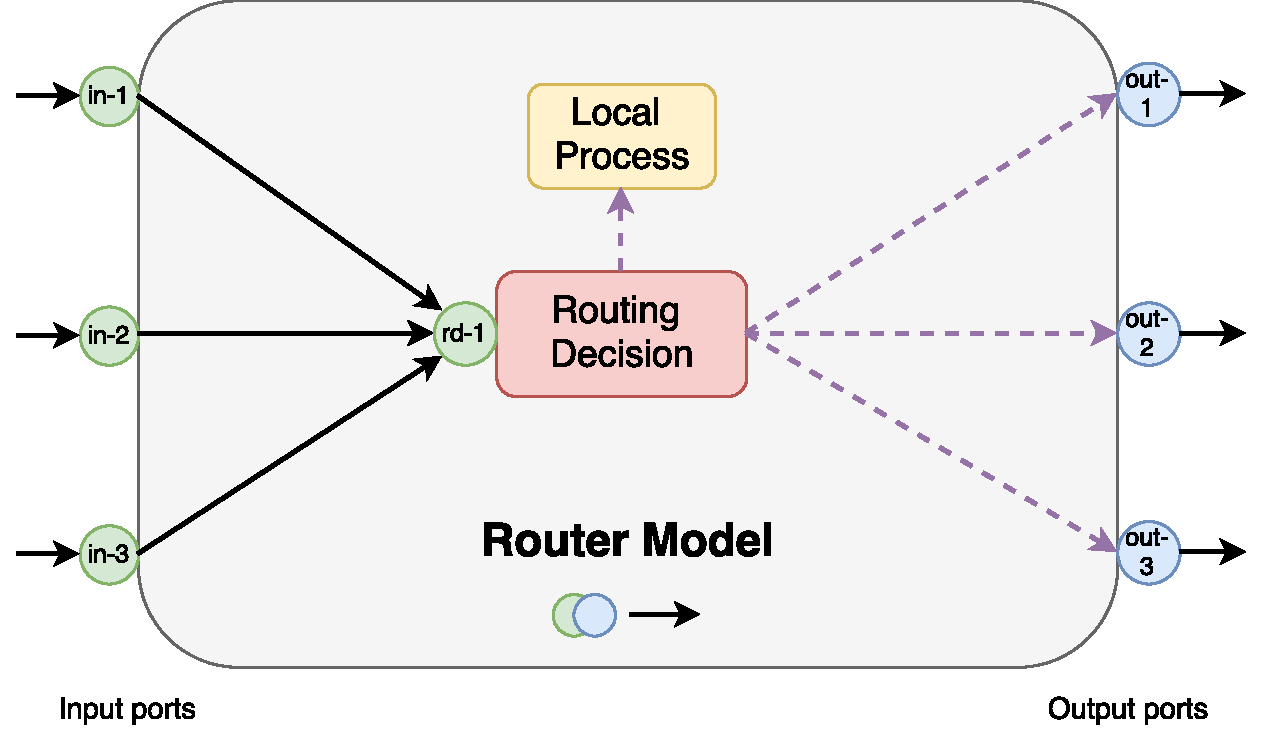
\includegraphics[scale=0.5]{assets/img/router-model}
  \sethlcolor{mathgray}
  \caption[Modelling a simple forwarding router.]{Modelling a simple router
  that only forwards packets based on its routing table. The model is given by
  \hl{$G=(V, E)$}, with \hl{$V=\{in_1, in_2, in_3, rd_1, out_1, out_2,
  out_3\}$}, \hl{$E=\{(in_1, rd_1), (in_2, rd_1), (in_3, rd_1)\}$}, and the
  \textbf{port} \hl{$rd_1$} having assigned the routing decision logic.}
  \label{fig:router-model}
\end{figure}

Firstly, we notice that the edges are directed and, thus, our model has
separate input and output ports.  Secondly, its only job is to route any
incoming packet irrespective of the input port it arrives on, so we connect all
input ports to an internal, hidden port, which is the input port of a
\emph{virtual device} called \textbf{routing decision}.  It is worth mentioning
that the same behaviour could have been achieved by assigning the instruction
\emph{Forward($rd_1$)} to all input ports instead of adding new edges to our
model.  Modularity and separation of concerns are some of the reasons behind
our choice.

The routing decision has an input port and forwards (dotted lines) the packet
to exactly one output port or to the local process.  One important thing to
notice is that the logic to iterate through an ordered list of IP prefixes can
be naively modelled as a sequence of \hltexttt{if/then/else} SEFL statements,
which means that its input port would suffice to express all this
functionality.  However, we model it as a standalone entity (through the red
square) to represent the idea of model encapsulation and components decoupling
by committing to well-defined \textbf{interfaces}.  For instance, if we decide
to use another model for routing decisions, which needs some intermmediate
ports, we can do so in isolation, as long as the \emph{contract} (input port,
output ports it forwards too, etc) is respected.

Finally, the \hltexttt{if/then/else} approach mentioned above is the most
straightforward one, but also the most inefficient way of implementing routing
table lookup. That being said, the more advanced and better performing ones do
not make the subject of this chapter.

\subsection{Running SymNet and interpreting the results}
\label{sub-sec:running-symnet}

\textbf{Running} SymNet is as simple as providing
\begin{enumerate*}[a)]
  \item the graph $G$ defined in the previous section that models the analyzed
    network, and
  \item an initial packet and a port to bootstrap symbolic execution with.
\end{enumerate*}

Owing to the one-to-many restriction, the graph $G$ is usually given as a
\textbf{Map} data structure (as opposed to a \textbf{Multimap}), with
\emph{from} ports as keys (therefore, each one will appear at most once) and
\emph{to} ports as values.  The set $V$ of nodes is simply the union of the set
of keys and the set of values in this Map.  The logic expressed using SEFL is
given as a separate data structure, mapping ports to their assigned SEFL
instructions.

What should the initial packet be?  The \emph{policy rule} that is being
verified should drive this choice
(\labelindexref{Section}{sec:network-verification}).  For instance, if we want
to ensure that an intranet is not reachable from the outside, we use purely
symbolic packets to ensure that all possible packets are verified.  On the
other hand, for more specific rules, such as verifying TCP reachability between
two nodes, we use concrete values for source and destination IP addresses, as
well as for protocol number, and leave all the rest unconstrained.

As previously mentioned, SymNet outputs an exhaustive list of flows together
with their constraints.  If the list is not a very large one, manually looking
through the resulting execution paths to ensure that the policy is respected is
a viable option.  This is often the case when a very constrained bootstrapping
packet is used.  However, more often than not this list is too large to be
inspected by hand.  For these cases, we have devised Scala matchers to use in
our automated testing suites.  In addition to that, as already discussed in
\labelindexref{Section}{sec:network-verification}, there are ongoing efforts to
integrate policy validation as part of the symbolic execution engine, by means
of various computation logics, such as CTL (Computation tree
logic)\abbrev{CTL}{Computation tree logic}.


\section{iptables}

Before delving into how we build a model of an iptables-enabled device using
SEFL and have it verified with SymNet, we must give an overview of what
iptables is and how it works.

We start with \textbf{netfilter} which is a framework provided by the Linux
kernel that allows various networking-related operations (such as packet
filtering, network address translation and other packet mangling) to be
implemented in the form of customized handlers.  Historically, the project
\emph{netfilter/iptables} was started by Rusty Russel in 1998 with the intent
to re-design and improve software packages that were part of previous versions
of the Linux kernel, such as ipchains and ipfwadm.

\textbf{iptables} is the user-space command line tool used to configure the
\emph{tables} defined by netfilter for IPv4 traffic (hence the name). Given
that it is the main application used by system administrators to define rules
for packet filtering/mangling, and having been an essential part of the initial
project that eventually evolved into today's framework, it is common to refer
through \emph{``iptables''} to the entire software stack that enables this, and
use \emph{``iptables''} and \emph{``netfilter''} interchangeably.  In fact, by
\emph{modelling iptables} we actually mean modelling the netfilter logic that
it triggers.


\subsection{Organization}

netfilter attains a modular internal organization by splitting rules into a
hierarchy of predefined \textbf{tables} and \textbf{chains}.  The latter can be
further extended by users, as depicted in
\labelindexref{Figure}{fig:iptables-hierarchy}.

\begin{figure}[h]
  \centering
  \captionsetup{justification=centering}
  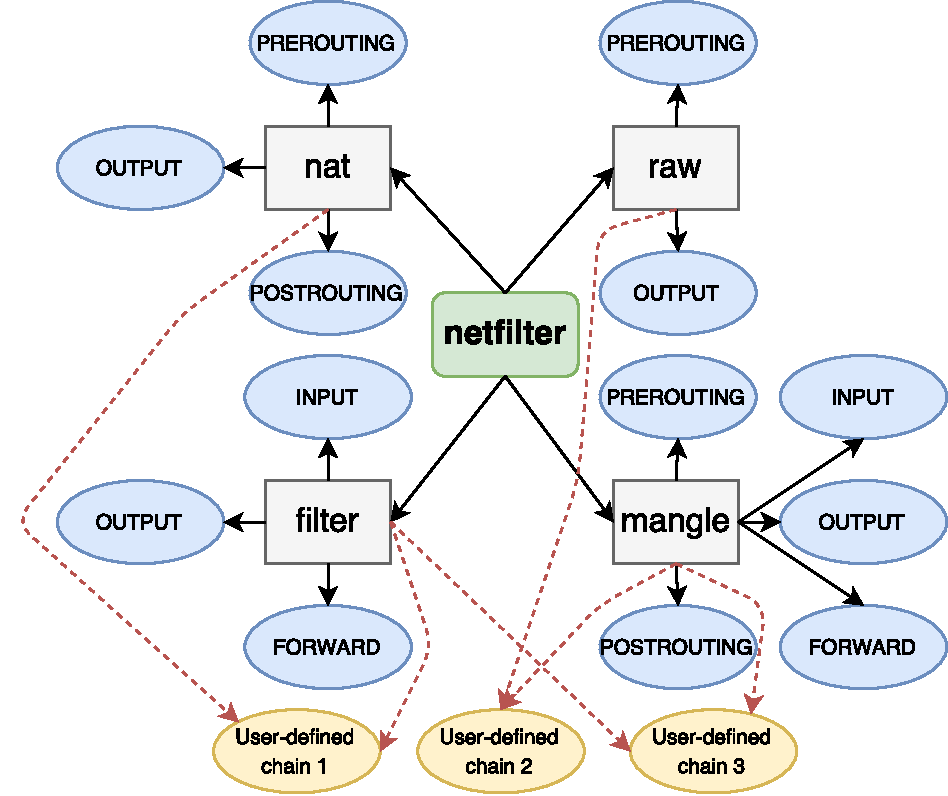
\includegraphics[scale=0.6]{assets/img/iptables-hierarchy}
  \caption[A visualization of the tables/chains hierarchy in netfilter.]{A
  visualization of the tables/chains hierarchy in netfilter. Note that there is
  at least one more table, \emph{security}, that is not included here.}
  \label{fig:iptables-hierarchy}
\end{figure}

\paragraph{Tables.}
Informally, tables are used to classify the rules based on their purpose.
Thus, each table is introduced to serve a specific function.  The most commonly
used ones are:
\begin{itemize}
  \item \textbf{filter} - for packet filtering only
  \item \textbf{nat} - for one-to-many NAT, port forwarding, masquerading,
    packet redirecting
  \item \textbf{mangle} - for specialized packet alteration; one feature that
    comes up often in practice is \emph{packet marking} which allows customized
    traffic handling by chains following it in the processing stack.
\end{itemize}

The lowercase spelling of table names is part of the convention adopted by
iptables/netfilter.  In terms of the netfilter implementation, each table
corresponds to a new hook in the hook system used to allow seamless extension
and hot-plugging.  Therefore, tables are traversed in a pre-established,
built-in \textbf{order}: raw, mangle, nat, filter.

\paragraph{Chains.}
As far as the chains are concerned, they specify the point in the
\textbf{processing stack} where the \emph{chain of rules} they represent will
be applied (\labelindexref{Figure}{fig:iptables-organization}).  There are 5
\textbf{built-in chains}:
\begin{itemize}
  \item PREROUTING - right after a packet is received and before any routing
    decision is made
  \item INPUT - for locally delivered packets
  \item FORWARD - all packets that transit this machine will be matched against
    the rules in this chain
  \item OUTPUT - packets sent from the machine itself will be visiting this
    chain
  \item POSTROUTING - packets enter this chain after the last routing decision
    is made and just before handing them off to the hardware
\end{itemize}

\begin{figure}[h]
  \centering
  \captionsetup{justification=centering}
  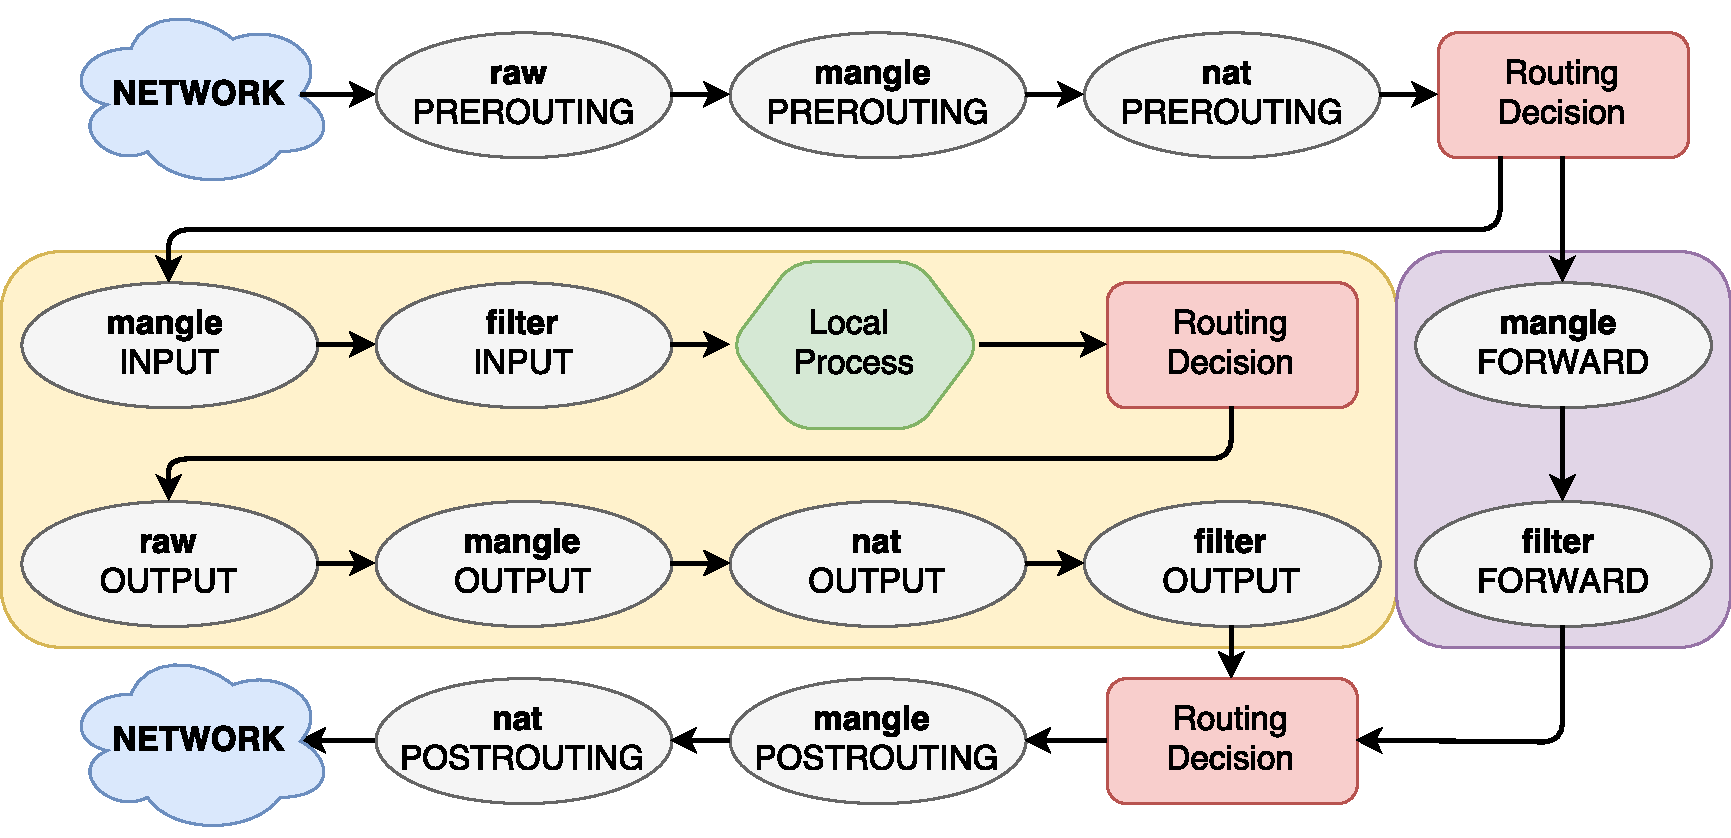
\includegraphics[scale=0.5]{assets/img/iptables-organization}
  \caption[A flowgraph showing the processing stack in netfilter/iptables.]{A
  flowgraph showing the usual processing stack in netfilter/iptables. The
  section on a yellow background is meaningful only for locally delivered or
  locally generated packets. The one on a purple background is traversed for
  all packets that only transit (are routed by) this machine.}
  \label{fig:iptables-organization}
\end{figure}

Additional chains can be defined; in netfilter/iptables terminology they are
called \textbf{user-defined chains}, and are featured in
\labelindexref{Figure}{fig:iptables-hierarchy}. The motivation behind their
existence is twofold:
\begin{itemize}
  \item To \textbf{share} logic between two built-in chains from the same table
    and avoid rule duplication.  For instance, we might want to apply the same
    \emph{filtering} rules both in the FORWARD chain and in the INPUT chain.
  \item To achieve some sort of \textbf{separation of concerns} when organizing
    the rules in a large chain. An example is a chain which only does SNAT, and
    the last rule of the POSTROUTING chain simply jumps to it.  In this way, we
    can short-circuit the traversal of this chain (i.e. \hltexttt{-j ACCEPT})
    for traffic that need not be SNAT-ed.
\end{itemize}

\paragraph{Rules.}
Tables and chains are only meant to organize the rules.  A rule is essentially
a \textbf{(match, action)} pair.  The first part, the \textbf{match}, is a
conjunction of zero or more \emph{predicates} that refer either to header
fields of the packet or to some local state associated with it.  The second
part, the \textbf{action}, specifies \emph{what} should happen with the packets
that match.  It can be followed by zero or more \emph{target parameters}. The
grammar that summarizes this is shown in
\labelindexref{Listing}{lst:rule-grammar}.

\begin{listing}
  \lstset{numbers=none, frame=single, basicstyle=\ttfamily,
    xleftmargin=0.15\textwidth, xrightmargin=0.15\textwidth
  }
\begin{lstlisting}
rule-specification = [matches...] [target]
match = -m matchname [per-match-options]
target = -j targetname [per-target-options]
\end{lstlisting}
  \caption{Grammar of an iptables rule, taken from the Linux manual pages.}
  \label{lst:rule-grammar}
\end{listing}

Rules in iptables feature an extensions-based design with separate extensions
for matches and targets. There are over 60 match extensions and around 40
target extensions.  Match extensions are \emph{activated} with the
\lstinline{-m/--match} flag followed by the extension name.
\labelindexref{Appendix}{app:iptables-extensions} summarizes some of the
extensions often used in practice.


\subsection{Relation with \emph{conntrack}}\label{sub-sec:conntrack}

Connection tracking (also known as \emph{the state machine}) is the mechanism
that allows a Linux box to relate incoming packets to tracked connections.
\textbf{conntrack} is the name of the kernel module that implements this
functionality.  Firewalls that include it are generally called \emph{stateful
firewalls}.

conntrack is part of netfilter and it is embedded in the processing stack
described in \labelindexref{Figure}{fig:iptables-organization}.  To be more
specific, it is called right after the raw table in the PREROUTING and OUTPUT
chains.  In fact, one of the purposes of the \textbf{raw} table is to allow
\textbf{skipping} connection tracking logic for certain traffic (i.e.
\lstinline{-j CT --notrack}).

Internally, for each connection, it holds two 5-tuples, one for each direction.
A 5-tuple contains protocol number, source IP, source port, destination IP and
destination port.  It recognizes four states:
\begin{itemize}
  \item \NEW.  It is the state of a connection when the first packet
    (within that connection) is seen.
  \item \ESTABLISHED.  In this state, traffic in both directions has been seen.
    A connection in state \NEW is promoted to state \ESTABLISHED once a reply
    packet is received.
  \item \RELATED.  A connection is tagged as \RELATED when it is related to
    another already \ESTABLISHED connection.  An example is a FTP data
    connection which is related to an established FTP control connection.
  \item \INVALID.  A connection switches to the \INVALID state if the packet
    cannot be identified, which could be caused by various system errors (going
    out of memory, etc).
\end{itemize}

By itself, conntrack is simply an aggregator for connection data.  It becomes
particularly powerful when the information it holds is used by iptables.  To do
so, the \textbf{conntrack} match extension must be loaded (i.e.
\lstinline{-m conntrack}).  The most common use-case is matching against the
connection state itself (i.e. \lstinline{-m conntrack --ctstate NEW}).  In
addition to the four states defined by the conntrack module, netfilter adds
three more \textbf{virtual} states to be used by iptables:
\begin{itemize}
  \item \UNTRACKED.  A state explicitly set in the raw table for untracked
    traffic, as shown above.
  \item \SNAT.  A state set for connections that have their packets Source
    NAT-ed by this machine.
  \item \DNAT.  A state set for connections for which this machine performs
    Destination NAT (e.g. port forwarding).
\end{itemize}

Besides the connection state, it is also possible to match against any of the
10 fields which are part of the two 5-tuples that are stored for every
connection.


\section{Summary}

We started this chapter by introducing the theoretical concept of \emph{network
verification} together with the most explored techniques to achieve it.  Once
we argued why static verification based on models built from network data
planes is the most promising approach, we switched our attention to symbolic
execution as a concrete verification procedure.

In the next section, we introduced SymNet and SEFL: the former is an
implementation of the previously discussed symbolic execution approach, while
the latter is a modelling language tailored for network processing.  We showed
how models are built using SEFL and how the output of SymNet can be
interpreted.

Finally, in the last section of this chapter we gave a detailed presentation of
iptables, its internal organization as well as its relation with connection
tracking.

In the next chapter we will make use of all the concepts accumulated so far to
build a model of an iptables-enabled device.
